% Author: Izaak Neutelings (July 2018)
% page 8 https://archive.org/details/StaticAndDynamicElectricity
% https://tex.stackexchange.com/questions/56353/extract-x-y-coordinate-of-an-arbitrary-point-on-curve-in-tikz
% https://tex.stackexchange.com/questions/412899/tikz-calculate-and-store-the-euclidian-distance-between-two-coordinates
\documentclass[border=3pt,tikz]{standalone}
\usepackage{amsmath} % for \dfrac
\usepackage{bm}
\usepackage{physics}
\usepackage{tikz,pgfplots}
\usetikzlibrary{angles,quotes} % for pic (angle labels)
\usetikzlibrary{calc}
\usetikzlibrary{decorations.markings}
\tikzset{>=latex} % for LaTeX arrow head

\usepackage{xcolor}
\colorlet{Ecol}{orange!90!black}
\colorlet{EcolFL}{orange!80!black}
\colorlet{veccol}{green!45!black}
\colorlet{EFcol}{red!60!black}
\tikzstyle{charged}=[top color=blue!20,bottom color=blue!40,shading angle=10]
\tikzstyle{darkcharged}=[very thin,top color=blue!60,bottom color=blue!80,shading angle=10]
\tikzstyle{charge+}=[very thin,top color=red!80,bottom color=red!80!black,shading angle=-5]
\tikzstyle{charge-}=[very thin,top color=blue!50,bottom color=blue!70!white!90!black,shading angle=10]
\tikzstyle{gauss surf}=[green!40!black,top color=green!2,bottom color=green!80!black!70,shading angle=5,fill opacity=0.5]
\tikzstyle{gauss lid}=[gauss surf,middle color=green!80!black!20,shading angle=40,fill opacity=0.6]
\tikzstyle{gauss dark}=[green!50!black,fill=green!60!black!70,fill opacity=0.8]
\tikzstyle{gauss line}=[green!40!black]
\tikzstyle{gauss dashed line}=[green!60!black!80,dashed,line width=0.2]
\tikzstyle{EField}=[->,thick,Ecol]
\tikzstyle{vector}=[->,thick,veccol]
\tikzstyle{normalvec}=[->,thick,blue!80!black!80]
\tikzstyle{EFieldLine}=[thick,EcolFL,decoration={markings,
          mark=at position 0.5 with {\arrow{latex}}},
          postaction={decorate}]
\tikzstyle{measure}=[fill=white,midway,outer sep=2]
\def\L{8}
\def\W{0.25}
\def\N{14}


\begin{document}


% ROD FIELD
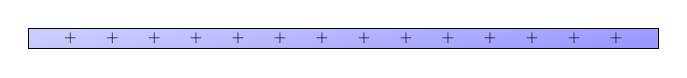
\begin{tikzpicture}
  \def\M{8}
  \def\ymax{\L/3}
    
  % ROD
  \draw[charged] (-\L/2,-\W/2) rectangle ++(\L,\W);
  \foreach \i [evaluate={\x=-\L/2+\i*\L/(\N+1);}] in {1,...,\N}{
    \node[scale=0.6] at (\x,0) {$+$};
  }
  
\end{tikzpicture}


% ROD SETUP
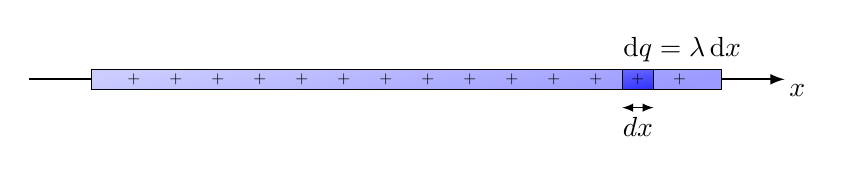
\begin{tikzpicture}
  
  \def\xmax{0.6*\L}
  \def\ymin{-0.18*\L}
  \def\ymax{0.5*\L}
  \def\x{0.342*\L}
  \def\dx{0.05*\L}
  \coordinate (O) at (0,0);
  \coordinate (X) at (\x,\W/2);
  
  % AXIS
  \draw[->,thick] (-\xmax,0) -- (\xmax,0) node[below right=-2] {$x$};
  
  % MEASURES
  \draw[<->] (\x,0.25*\ymin) --++ (\dx,0) node[midway,below] {$dx$};
  
  % ROD
  \draw[charged] (-\L/2,-\W/2) rectangle ++(\L,\W);
  \draw[darkcharged] (\x,-\W/2) rectangle ++(\dx,\W)
    node[midway,right=16,above=3] {$\dd{q}=\lambda\dd{x}$};
  \foreach \i [evaluate={\x=-\L/2+\i*\L/(\N+1);}] in {1,...,\N}{
    \node[scale=0.6] at (\x,0) {$+$};
  }
  
\end{tikzpicture}


% ROD ELECTRIC FIELD HORIZONTAL
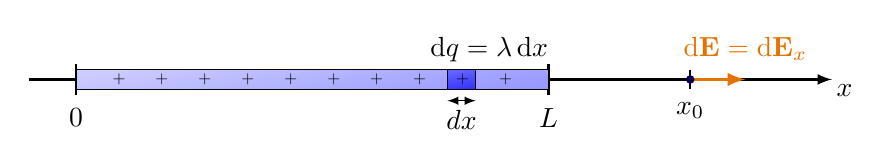
\begin{tikzpicture}
  \def\L{6}
  \def\N{10}
  \def\xmin{-0.1*\L}
  \def\xmax{1.6*\L}
  \def\ymin{-0.18*\L}
  \def\ymax{0.5*\L}
  \def\x{0.786*\L}
  \def\xz{1.3*\L}
  \def\dx{0.06*\L}
  \coordinate (O) at (0,0);
  \coordinate (X) at (\x,\W/2);
  \coordinate (P) at (\xz,0);
  
  % AXIS
  \draw[->,thick] (\xmin,0) -- (\xmax,0) node[below right=-2] {$x$};
  \draw[thick] (0,0.8*\W) --++ (0,-1.6*\W) node[below=1] {$0$};
  \draw[thick] (\L,0.8*\W) --++ (0,-1.6*\W) node[below=1] {$L$};
  \draw[thick] (\xz,0.5*\W) --++ (0,-1.0*\W) node[below=1] {$x_0$};
  
  % MEASURES
  \draw[<->] (\x,0.25*\ymin) --++ (\dx,0) node[midway,below] {$dx$};
  
  % ROD
  \draw[charged] (0,-\W/2) rectangle ++(\L,\W);
  \draw[darkcharged] (\x,-\W/2) rectangle ++(\dx,\W)
    node[midway,right=10,above=3] {$\dd{q}=\lambda\dd{x}$};
  \foreach \i [evaluate={\x=\i*\L/(\N+1);}] in {1,...,\N}{
    \node[scale=0.6] at (\x,0) {$+$};
  }
  
  % ELECTRIC FIELD
  \draw[EField,very thick] (P) --++ (0.7,0) node[above=3] {$\dd{\vb{E}} = \dd{\vb{E}_x}$};
  \node[fill=blue!30!black,circle,inner sep=1.1] (P') at (P) {};
  
\end{tikzpicture}


% ROD ELECTRIC FIELD VERTICAL
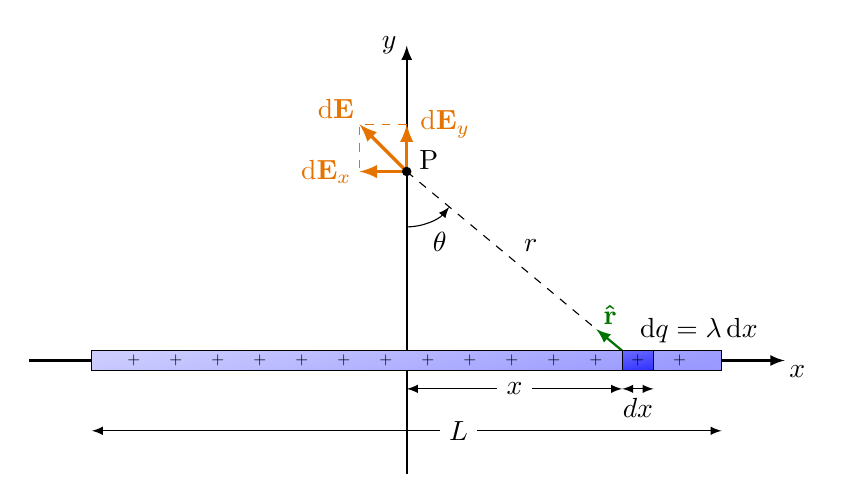
\begin{tikzpicture}
  
  \def\xmax{0.6*\L}
  \def\ymin{-0.18*\L}
  \def\ymax{0.5*\L}
  \def\x{0.342*\L}
  \def\dx{0.05*\L}
  \coordinate (O) at (0,0);
  \coordinate (P) at (0,{0.6*\ymax});
  \coordinate (X) at (\x,\W/2);
  
  % AXIS
  \draw[->,thick] (-\xmax,0) -- (\xmax,0) node[below right=-2] {$x$};
  \draw[->,thick] (0,\ymin) -- (0,\ymax) node[left] {$y$};
  
  % MEASURES
  %\draw[<->] (0,0.2*\ymax) --++ (\x,0) node[midway,above] {$x$};
  \draw[<->] (    0,0.25*\ymin) --++ (\x,0) node[measure] {$x$};
  \draw[<->] (   \x,0.25*\ymin) --++ (\dx,0) node[midway,below] {$dx$};
  \draw[<->] (-\L/2,0.62*\ymin) --++ (\L,0) node[measure,right=10] {$L$};
  
  % VECTORS
  \draw[EField,very thick] (P) --++ ( 0.0,0.6) node[right=1] {$\dd{\vb{E}_y}$};
  \draw[EField,very thick] (P) --++ (-0.6,0.0) node[left=-1] {$\dd{\vb{E}_x}$};
  \draw[EField,very thick] (P) --++ (-0.6,0.6) node[above left=-2] {$\dd{\vb{E}}$};
  \draw[EField,-,dashed,thin] (P) ++ (0,0.6) --++ (-0.6,0) --++ (0,-0.6);
  
  % POINT
  \fill (P) circle (0.06) node[above=4,right=1] {P};
  \draw[dashed] (P) -- (X) node[midway,above right] {$r$};
  \draw pic[->,"$\theta$",draw=black,angle radius=20,angle eccentricity=1.4] {angle = O--P--X};
  \draw[vector] (X) -- ($(X)!0.12!(P)$) node[right=5,above=-2] {$\vu{r}$};
  
  % ROD
  \draw[charged] (-\L/2,-\W/2) rectangle ++(\L,\W);
  \draw[darkcharged] (\x,-\W/2) rectangle ++(\dx,\W)
    node[midway,right=22,above=3] {$\dd{q}=\lambda \dd{x}$};
  \foreach \i [evaluate={\x=-\L/2+\i*\L/(\N+1);}] in {1,...,\N}{
    \node[scale=0.6] at (\x,0) {$+$};
  }
  
\end{tikzpicture}


% ROD FIELD
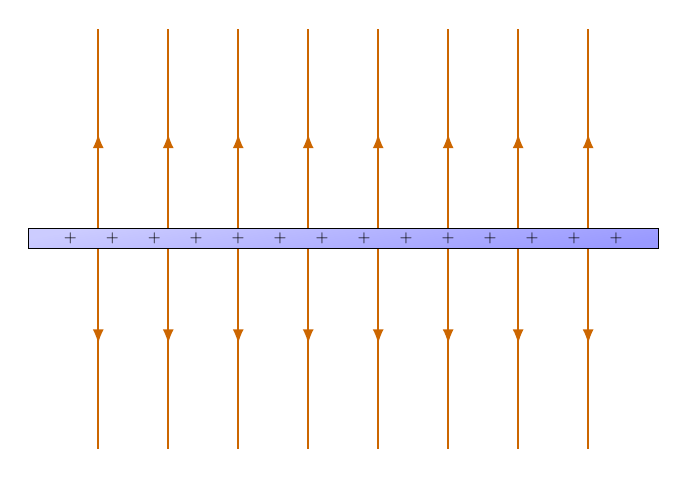
\begin{tikzpicture}
  \def\M{8}
  \def\ymax{\L/3}
  
  % ELECTRIC FIELD
  \foreach \i [evaluate={\x=-\L/2+\i*\L/(\M+1);}] in {1,...,\M}{
    \draw[EFieldLine] (\x,0) --++ (0,+\ymax);
    \draw[EFieldLine] (\x,0) --++ (0,-\ymax);
  }
  
  % ROD
  \draw[charged] (-\L/2,-\W/2) rectangle ++(\L,\W);
  \foreach \i [evaluate={\x=-\L/2+\i*\L/(\N+1);}] in {1,...,\N}{
    \node[scale=0.6] at (\x,0) {$+$};
  }
  
\end{tikzpicture}


% ROD REALISTIC FIELD with GAUSS
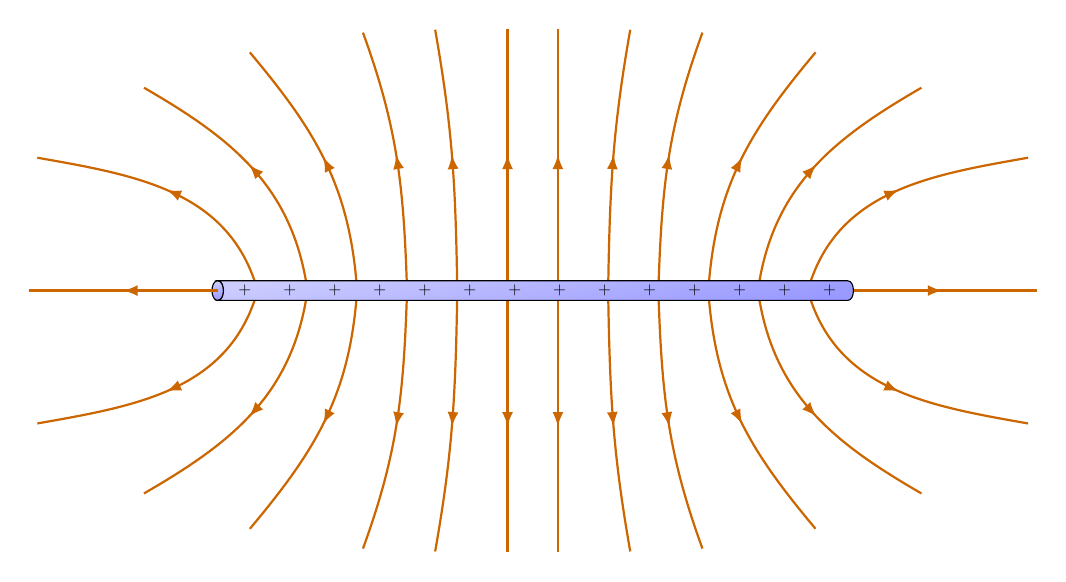
\begin{tikzpicture}
  \def\M{8}
  \def\R{0.4*\L}
  \def\g{0.2*\R}
  \def\G{0.6*\R}
  \def\a{0.305*\L}
  \coordinate (L)  at (-\a,0);
  \coordinate (R)  at (+\a,0);
  \coordinate (TL) at (-\a,\G);
  \coordinate (TR) at (+\a,\G);
  \coordinate (BL) at (-\a,-\G);
  \coordinate (BR) at (+\a,-\G);
  \def\angle#1{{\y*(\ang+\x*#1)}}
  
  \draw[charged] (-\L/2,-\W/2) to[out=180,in=180] ++ (0,\W) to[out=0,in=0] cycle;
  
  % FIELD LINES
  \foreach \y in {-1,1}{
    \foreach \x [evaluate={\ang=(1-\x)*90;}] in {-1,1}{
      \message{\y,\x,\ang ^^J}
      \draw[EFieldLine] (\x*0.040*\L,\y*\W/2) to[out=\angle{90},in=\angle{ -90}] ++(\angle{90}:\R);
      \draw[EFieldLine] (\x*0.120*\L,\y*\W/2) to[out=\angle{89},in=\angle{-100}] ++(\angle{85}:\R);
      \draw[EFieldLine] (\x*0.200*\L,\y*\W/2) to[out=\angle{88},in=\angle{-110}] ++(\angle{80}:\R);
      \draw[EFieldLine] (\x*0.280*\L,\y*\W/2) to[out=\angle{85},in=\angle{-130}] ++(\angle{65}:\R);
      \draw[EFieldLine] (\x*0.360*\L,\y*\W/2) to[out=\angle{80},in=\angle{-150}] ++(\angle{50}:\R);
      \draw[EFieldLine] (\x*0.440*\L,0.35*\y*\W) to[out=\angle{72},in=\angle{-170}] ++(\angle{30}:\R);
    }
  }
  \draw[EFieldLine] (\L/2,0) --++ (0:0.75*\R);
  \draw[EFieldLine] (-\L/2,0) --++ (180:0.75*\R);
  
  % ROD
  \draw[charged] (-\L/2,-\W/2) --++(\L,0) to[out=0,in=0] ++ (0,\W) --++ (-\L,0) to[out=0,in=0] cycle;
  \foreach \i [evaluate={\x=-\L/2+(\i-0.4)*\L/\N;}] in {1,...,\N}{
    \node[scale=0.6] at (\x,0) {$+$};
  }
  
\end{tikzpicture}


% ROD SIDEVIEW
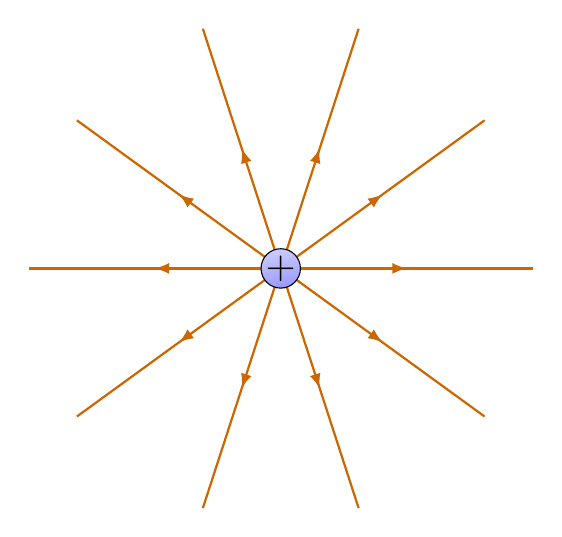
\begin{tikzpicture}
  \def\M{10}
  \def\R{0.4*\L}
  \def\G{0.8*\R}
  
  % ELECTRIC FIELD
  \foreach \i [evaluate={\angle=\i*360/\M;}] in {1,...,\M}{
    \draw[EFieldLine] (0,0) --++ (\angle:\R);
  }
  
  % ROD
  \draw[charged] (0,0) circle (\W) node[scale=1.4] {$+$};
  
\end{tikzpicture}


% ROD FIELD 3D
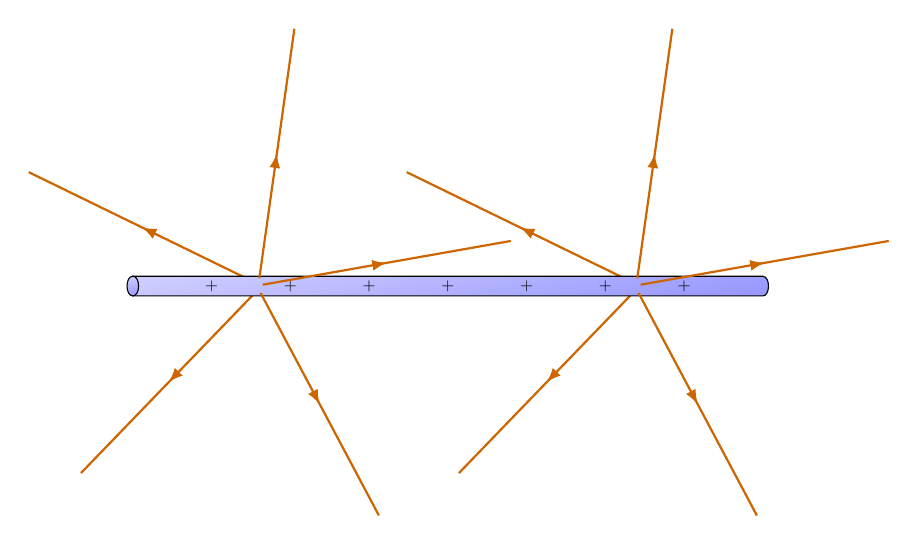
\begin{tikzpicture}
  \def\N{7}
  \def\M{5}
  \def\R{0.4*\L}
  \def\g{0.2*\R}
  \def\G{0.6*\R}
  \def\a{0.33*\L}
  \coordinate (L)  at (-\a,0);
  \coordinate (R)  at (+\a,0);
  \coordinate (TL) at (-\a,\G);
  \coordinate (TR) at (+\a,\G);
  \coordinate (BL) at (-\a,-\G);
  \coordinate (BR) at (+\a,-\G);
  
  % FIELD LINES
  \foreach \i [evaluate={\ang=10+\i*360/\M;}] in {2,3}{
    \draw[EFieldLine] (-0.3*\L,0)++({0.2*\W*cos(\ang)},{0.4*\W*sin(\ang)}) --++ (\ang:\R);
    \draw[EFieldLine] (+0.3*\L,0)++({0.2*\W*cos(\ang)},{0.4*\W*sin(\ang)}) --++ (\ang:\R);
  }
  
  % ROD
  \draw[charged] (-\L/2,-\W/2) --++(\L,0) to[out=0,in=0] ++ (0,\W) --++ (-\L,0) -- cycle;
  \draw[charged] (-\L/2,-\W/2) to[out=180,in=180] ++ (0,\W) to[out=0,in=0] cycle;
  \foreach \i [evaluate={\x=-\L/2+\i*\L/(\N+1);}] in {1,...,\N}{
    \node[scale=0.6] at (\x,0) {$+$};
  }
  
  % FIELD LINES
  \foreach \i [evaluate={\ang=10+\i*360/\M;}] in {4,5,1}{
    \draw[EFieldLine] (-0.3*\L,0)++({0.2*\W*cos(\ang)},{0.4*\W*sin(\ang)}) --++ (\ang:\R);
    \draw[EFieldLine] (+0.3*\L,0)++({0.2*\W*cos(\ang)},{0.4*\W*sin(\ang)}) --++ (\ang:\R);
  }
  
\end{tikzpicture}


% ROD GAUSS
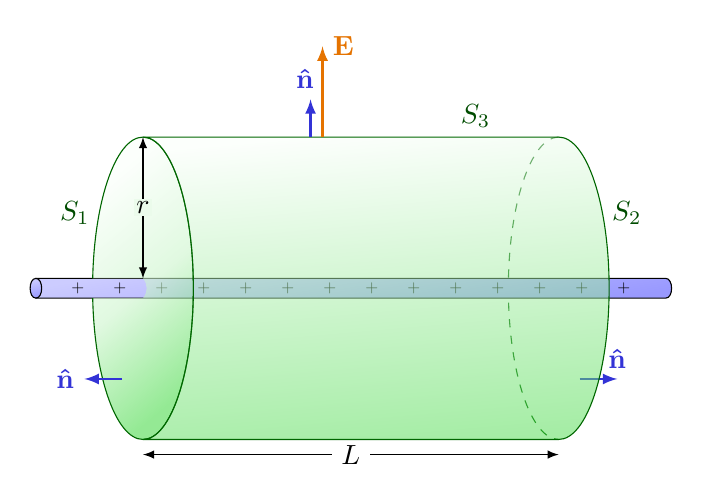
\begin{tikzpicture}
  \def\M{8}
  \def\R{0.4*\L}
  \def\g{0.2*\R}
  \def\G{0.6*\R}
  \def\a{0.33*\L}
  \coordinate (L)  at (-\a,0);
  \coordinate (R)  at (+\a,0);
  \coordinate (TL) at (-\a,\G);
  \coordinate (TR) at (+\a,\G);
  \coordinate (BL) at (-\a,-\G);
  \coordinate (BR) at (+\a,-\G);
  
  % GAUSS BEHIND
  \draw[gauss line,dashed] (TR) arc (90:270:{\g} and {\G});
  
  % ROD
  \draw[charged] (-\L/2,-\W/2) --++(\L,0) to[out=0,in=0] ++ (0,\W) --++ (-\L,0) -- cycle;
  \draw[charged] (-\L/2,-\W/2) to[out=180,in=180] ++ (0,\W) to[out=0,in=0] cycle;
  \foreach \i [evaluate={\x=-\L/2+\i*\L/(\N+1);}] in {1,...,\N}{
    \node[scale=0.6] at (\x,0) {$+$};
  }
  \begin{scope}
    \clip (-\L/2,-0.5*\W)
      --++ (\L/2-\a,0) to[out=50,in=-50] ++(0,1.0*\W) --++ (-\L/2+\a,0) --++ (0,\G)
      --++ (\L-2*\a,0) --++ (0,{-2*(\G+\W)}) --++ (-\L+2*\a,0) -- cycle;
    \draw[gauss lid] (L) ellipse ({\g} and {\G});
  \end{scope}
  
  
  % GAUSS IN FRONT
  \draw[<->] (-\a,\W/2) -- (-\a,\G) node[measure,fill=green!80!black!8,inner sep=1,outer sep=0] {$r$};
  \draw[<->] (-\a,-1.1*\G) -- (\a,-1.1*\G) node[measure] {$L$};
  \draw[normalvec] (-1.1*\a,-0.6*\G) --++ (-0.25*\G,0) node[left] {$\vu{n}$};
  \draw[normalvec] (+1.1*\a,-0.6*\G) --++ (+0.25*\G,0) node[above] {$\vu{n}$};
  \draw[gauss surf]
    (BL) arc (-90:90:{\g} and {\G}) --
    (TR) arc (90:-90:{\g} and {\G}) -- cycle;
  \draw[normalvec] (-0.064*\L,\G) --++ (0,0.25*\G) node[left=2,above] {$\vu{n}$};
  \draw[->,thick,Ecol] (-0.045*\L,\G) --++ (0,0.6*\G) node[right] {$\vb{E}$};
  
  % LABELS
  \node[left,green!30!black] at ($(-\a,0)+(150:{\g} and {\G})$) {$S_1$};
  \node[right,green!30!black] at ($(\a,0)+(30:{\g} and {\G})$) {$S_2$};
  \node[above,green!30!black] at (0.6*\a,\G) {$S_3$};
  
\end{tikzpicture}


% ROD REALISTIC FIELD with GAUSS
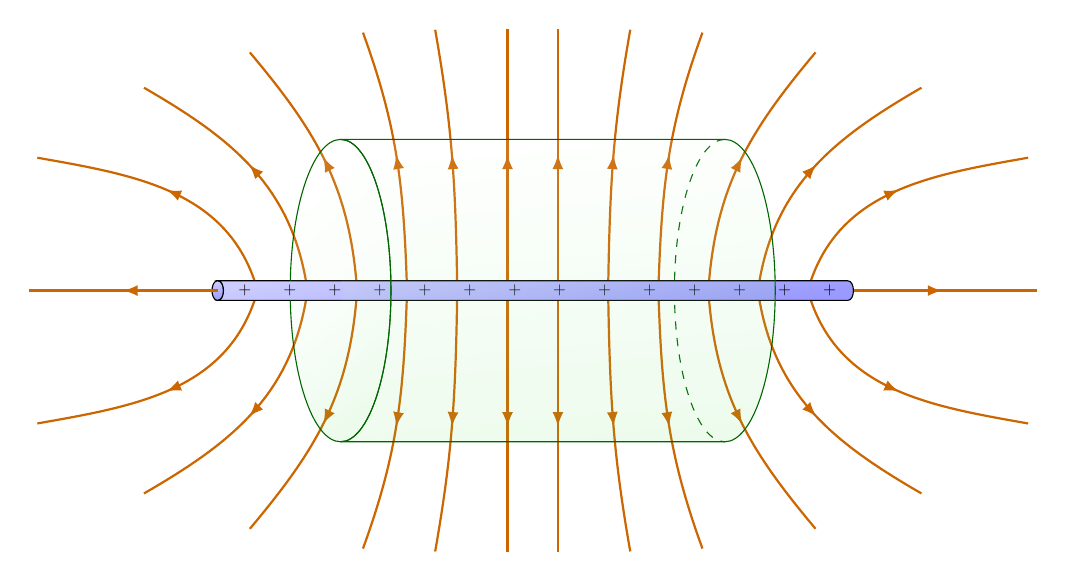
\begin{tikzpicture}
  \def\M{8}
  \def\R{0.4*\L}
  \def\g{0.2*\R}
  \def\G{0.6*\R}
  \def\a{0.305*\L}
  \coordinate (L)  at (-\a,0);
  \coordinate (R)  at (+\a,0);
  \coordinate (TL) at (-\a,\G);
  \coordinate (TR) at (+\a,\G);
  \coordinate (BL) at (-\a,-\G);
  \coordinate (BR) at (+\a,-\G);
  \def\angle#1{{\y*(\ang+\x*#1)}}
  
  % GAUSS BEHIND
  \draw[gauss line,dashed] (TR) arc (90:270:{\g} and {\G});
  
  \draw[charged] (-\L/2,-\W/2) to[out=180,in=180] ++ (0,\W) to[out=0,in=0] cycle;
  
  % FIELD LINES
  \foreach \y in {-1,1}{
    \foreach \x [evaluate={\ang=(1-\x)*90;}] in {-1,1}{
      \message{\y,\x,\ang ^^J}
      \draw[EFieldLine] (\x*0.040*\L,\y*\W/2) to[out=\angle{90},in=\angle{ -90}] ++(\angle{90}:\R);
      \draw[EFieldLine] (\x*0.120*\L,\y*\W/2) to[out=\angle{89},in=\angle{-100}] ++(\angle{85}:\R);
      \draw[EFieldLine] (\x*0.200*\L,\y*\W/2) to[out=\angle{88},in=\angle{-110}] ++(\angle{80}:\R);
      \draw[EFieldLine] (\x*0.280*\L,\y*\W/2) to[out=\angle{85},in=\angle{-130}] ++(\angle{65}:\R);
      \draw[EFieldLine] (\x*0.360*\L,\y*\W/2) to[out=\angle{80},in=\angle{-150}] ++(\angle{50}:\R);
      \draw[EFieldLine] (\x*0.440*\L,0.35*\y*\W) to[out=\angle{72},in=\angle{-170}] ++(\angle{30}:\R);
    }
  }
  \draw[EFieldLine] (\L/2,0) --++ (0:0.75*\R);
  \draw[EFieldLine] (-\L/2,0) --++ (180:0.75*\R);
  
  % ROD
  \draw[charged] (-\L/2,-\W/2) --++(\L,0) to[out=0,in=0] ++ (0,\W) --++ (-\L,0) to[out=0,in=0] cycle;
  \foreach \i [evaluate={\x=-\L/2+(\i-0.4)*\L/\N;}] in {1,...,\N}{
    \node[scale=0.6] at (\x,0) {$+$};
  }
  \begin{scope}
    \clip (-\L/2,-0.5*\W)
      --++ (\L/2-\a,0) to[out=50,in=-50] ++(0,1.0*\W) --++ (-\L/2+\a,0) --++ (0,\G)
      --++ (\L-2*\a,0) --++ (0,{-2*(\G+\W)}) --++ (-\L+2*\a,0) -- cycle;
    \draw[gauss lid,fill opacity=0.1] (L) ellipse ({\g} and {\G});
  \end{scope}
  
  % GAUSSIAN SURFACE FRONT
  \draw[gauss surf,fill opacity=0.1]
    (BL) arc (-90:90:{\g} and {\G}) --
    (TR) arc (90:-90:{\g} and {\G}) -- cycle;
  
\end{tikzpicture}


% ROD GAUSS SIDEVIEW
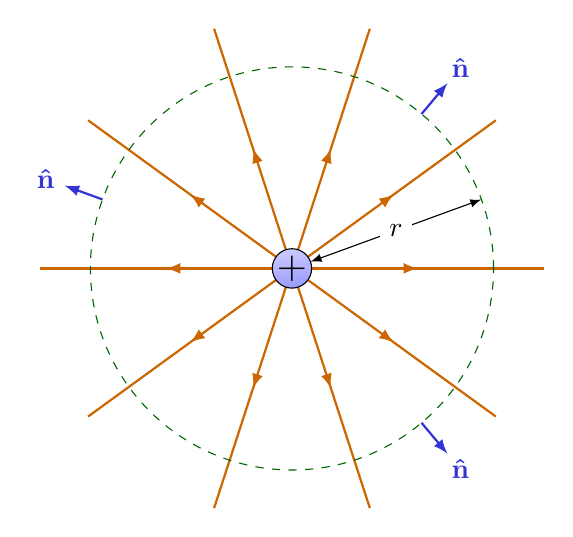
\begin{tikzpicture}
  \def\M{10}
  \def\R{0.4*\L}
  \def\G{0.8*\R}
  
  % ELECTRIC FIELD
  \foreach \i [evaluate={\angle=\i*360/\M;}] in {1,...,\M}{
    \draw[EFieldLine] (0,0) --++ (\angle:\R);
  }
  
  % ROD
  \draw[charged] (0,0) circle (\W) node[scale=1.4] {$+$};
  
  % GAUSSIAN SURFACE
  \draw[gauss line,dashed] (0,0) circle (\G);
  \draw[<->] (0,0) ++ (20:\W) -- (20:\G) node[measure] {$r$};
  \foreach \angle in {50,160,310}{
    \draw[normalvec] (0,0) ++ (\angle:\G) --++ (\angle:0.2*\G);
    \node[normalvec] at (\angle:1.30*\G) {$\vu{n}$};
  }
  
\end{tikzpicture}


\end{document}
